\documentclass[11pt,a4paper]{article}
\usepackage[margin=1.8cm]{geometry}
\usepackage[T1]{fontenc}
\usepackage[utf8]{inputenc}
\usepackage{lmodern}
\usepackage{microtype}
\usepackage{booktabs,longtable,tabularx,array,multirow}
\usepackage{graphicx}
\usepackage{xcolor}
\usepackage{xurl}
\usepackage{hyperref}
\usepackage{enumitem}
\usepackage{fancyhdr}
\usepackage{titlesec}
\usepackage{tcolorbox}
\tcbuselibrary{breakable,skins}
\usepackage{tikz}
\usetikzlibrary{arrows.meta,positioning,shapes.geometric,fit}
\usepackage{amsmath}
\usepackage{caption}
\usepackage{float}
\usepackage{setspace}
\usepackage{lastpage}

\definecolor{navy}{HTML}{12324A}
\definecolor{bluebox}{HTML}{EAF3F8}
\definecolor{greenbox}{HTML}{ECF7F1}
\definecolor{amberbox}{HTML}{FFF5DD}
\definecolor{redbox}{HTML}{FDECEC}
\definecolor{graybox}{HTML}{F4F5F6}
\definecolor{rulegray}{HTML}{D7DCE0}

\hypersetup{colorlinks=true,linkcolor=navy,urlcolor=navy,citecolor=navy,pdftitle={IELTS Band 9 Output Mastery Supplement}}
\setlength{\headheight}{14pt}
\Urlmuskip=0mu plus 1mu
\pagestyle{fancy}
\fancyhf{}
\lhead{IELTS Band 9 Output Mastery}
\rhead{Writing + Speaking Supplement}
\cfoot{\thepage\ / \pageref{LastPage}}
\renewcommand{\headrulewidth}{0.3pt}

\titleformat{\section}{\Large\bfseries\color{navy}}{\thesection}{0.6em}{}
\titleformat{\subsection}{\large\bfseries\color{navy}}{\thesubsection}{0.6em}{}
\titleformat{\subsubsection}{\normalsize\bfseries}{\thesubsubsection}{0.6em}{}
\setlist[itemize]{topsep=3pt,itemsep=2pt,leftmargin=1.3em}
\setlist[enumerate]{topsep=3pt,itemsep=2pt,leftmargin=1.5em}
\setlength{\parindent}{0pt}
\setlength{\parskip}{5pt}
\renewcommand{\arraystretch}{1.25}

\newtcolorbox{keybox}[1][]{colback=bluebox,colframe=navy,boxrule=0.6pt,arc=2mm,breakable,title=#1,fonttitle=\bfseries}
\newtcolorbox{practicebox}[1][]{colback=greenbox,colframe=green!45!black,boxrule=0.6pt,arc=2mm,breakable,title=#1,fonttitle=\bfseries}
\newtcolorbox{warningbox}[1][]{colback=redbox,colframe=red!55!black,boxrule=0.6pt,arc=2mm,breakable,title=#1,fonttitle=\bfseries}
\newtcolorbox{aibox}[1][]{colback=amberbox,colframe=orange!60!black,boxrule=0.6pt,arc=2mm,breakable,title=#1,fonttitle=\bfseries}
\newtcolorbox{evidencebox}[1][]{colback=graybox,colframe=gray!65!black,boxrule=0.5pt,arc=2mm,breakable,title=#1,fonttitle=\bfseries}
\newcommand{\src}[1]{\textsuperscript{[#1]}}

\begin{document}

\begin{titlepage}
\centering
\vspace*{2.2cm}
{\Huge\bfseries\color{navy} IELTS Band 9 Output Mastery\par}
\vspace{0.4cm}
{\LARGE Writing, Speaking, Free Tools, AI Workflows, and Score Strategy\par}
\vspace{0.8cm}
{\large A deep supplement to the pronunciation-first master report\par}
\vfill
\begin{tcolorbox}[width=0.88\textwidth,colback=bluebox,colframe=navy,arc=2mm]
\textbf{Profile used for planning:} advanced English learner; current profile from the project context is Reading 9, Listening 9, Writing 7, Speaking 7.5. The strategic objective is an overall IELTS 9 while developing genuinely advanced English rather than test tricks.
\end{tcolorbox}
\vspace{0.5cm}
\begin{tcolorbox}[width=0.88\textwidth,colback=greenbox,colframe=green!45!black,arc=2mm]
\textbf{Free-only rule:} every recommended app or software workflow in this report can be used without paying, without a trial, and without buying credits. Where a product has paid features, only its permanently free function is recommended. Local open-source alternatives are preferred.
\end{tcolorbox}
\vfill
{\small Research and tool availability checked against sources available in August 2026.}
\end{titlepage}

\tableofcontents
\newpage

\section*{Executive Summary}
\addcontentsline{toc}{section}{Executive Summary}

\begin{keybox}[The single most important score correction]
An overall average of \textbf{8.5 does not round to 9}. IELTS reports the mean of the four section scores, rounded to the nearest half or whole band; an average ending in .75 rounds up to the next whole band. Therefore the practical threshold for an overall Band 9 is \textbf{8.75}.\src{1}

With Reading 9 and Listening 9 held constant, Writing 8.5 + Speaking 8.5 produces an average of 8.75 and therefore an overall Band 9. Writing 8 + Speaking 9 also reaches 8.75. This makes \textbf{reliable 8.5-level productive performance} a strategically sufficient target, although a cushion above the threshold is safer.
\end{keybox}

\begin{warningbox}[There is no legitimate way to guarantee Band 9]
No teacher, app, AI model, or study schedule can guarantee a future IELTS score. Writing and Speaking are human-rated productive tasks, and performance varies by prompt, day, fatigue, and sampling. The goal of this report is therefore to \textbf{maximize probability and reduce avoidable variance}: use official descriptors, repeated timed samples, delayed transfer tests, multiple feedback sources, and a safety margin above the minimum score combination.
\end{warningbox}

\textbf{What changes from the earlier plan?}
\begin{itemize}
\item Band 9 does \emph{not} literally require zero errors or zero hesitation. Official Speaking Band 9 allows very occasional repetition/self-correction and native-speaker-like mistakes; Writing Band 9 allows extremely rare minor errors.\src{2}\src{3}
\item Writing improvement should not be based on writing hundreds of first drafts. Research on feedback supports cycles of drafting, feedback, revision, and transfer; combined surface and deep feedback is more useful than correction alone.\src{11}\src{12}
\item Speaking fluency can benefit from task repetition, but repetition should be followed by a \emph{new} task to test transfer. Recent meta-analytic work finds positive effects of oral task repetition, while the 4/3/2 technique appears especially useful for fluency rather than guaranteed accuracy gains.\src{14}\src{15}
\item AI should be a critic, generator, transcriber, and organizer -- \textbf{not an IELTS examiner substitute}. Recent evidence finds small-to-moderate average benefits from automated/AI feedback, with substantial heterogeneity and limited transfer in some studies.\src{12}\src{13}
\end{itemize}

\section{Score Mathematics: How an Overall 9 Actually Happens}

IELTS calculates the overall score as the mean of Listening, Reading, Writing, and Speaking, then rounds to the nearest half or whole band. A mean ending in .25 rounds upward to the next half band; a mean ending in .75 rounds upward to the next whole band.\src{1}

\begin{table}[H]
\centering
\caption{Strategic score combinations if Reading = 9 and Listening = 9}
\begin{tabular}{cccccc}
\toprule
Reading & Listening & Writing & Speaking & Mean & Overall \\
\midrule
9.0 & 9.0 & 8.5 & 8.5 & 8.75 & \textbf{9.0} \\
9.0 & 9.0 & 8.0 & 9.0 & 8.75 & \textbf{9.0} \\
9.0 & 9.0 & 9.0 & 8.0 & 8.75 & \textbf{9.0} \\
9.0 & 9.0 & 8.5 & 9.0 & 8.875 & \textbf{9.0} \\
9.0 & 9.0 & 8.0 & 8.5 & 8.625 & 8.5 \\
\bottomrule
\end{tabular}
\end{table}

\begin{figure}[H]
\centering
\includegraphics[width=0.80\textwidth]{overall_band_heatmap.png}
\caption{Rounded overall score as Writing and Speaking vary, with Reading and Listening fixed at 9. The plotted values are computed directly from the official rounding rule.}
\end{figure}

\begin{practicebox}[The risk-managed target]
Do not train to ``barely touch 8.75.'' A better practice target is a rolling set of timed performances that would average roughly \textbf{8.875 or above} if converted to band-equivalent scores. This is not an IELTS rule; it is a risk-management inference designed to absorb ordinary test-day variation.
\end{practicebox}

\section{What Band 9 Writing and Speaking Really Require}

\subsection{Writing}
IELTS Writing uses four equally weighted criteria within each task: Task Achievement for Task 1 or Task Response for Task 2, Coherence and Cohesion, Lexical Resource, and Grammatical Range and Accuracy. Task 2 carries more weight than Task 1 in the final Writing score.\src{4}\src{5}

At Band 9, the public descriptors emphasize: fully and appropriately fulfilling the task, deep exploration and well-supported development, effortless progression, precise and natural vocabulary, and wide grammatical control. The descriptors still permit \emph{extremely rare} minor lapses or errors.\src{3}

\subsection{Speaking}
Speaking is equally weighted across Fluency and Coherence, Lexical Resource, Grammatical Range and Accuracy, and Pronunciation.\src{2}\src{6}

Band 9 is not ``never pause.'' It is closer to this: pauses are for content rather than searching for basic language; topic development remains coherent; lexical choices are precise and idiomatic; grammar is consistently controlled apart from native-like slips; and pronunciation/connected speech make the speaker effortless to understand.\src{2}

\begin{keybox}[Band 8.5 is not a separate public descriptor]
IELTS publishes whole-band descriptors. A half band generally means the performance falls between adjacent descriptor levels. Therefore your operational target should be: \textbf{demonstrate Band 9 features frequently while avoiding Band 7 limiting features and keeping Band 8 weaknesses genuinely occasional}. This is a training interpretation, not an official formula.
\end{keybox}

\section{Writing 7 to 8.5/9: A Deliberate-Practice System}

\subsection{Why Band 7 often stalls}
A Band 7 writer usually has enough English to produce clear essays, so improvement becomes less about acquiring more vocabulary and more about eliminating \emph{systematic} weaknesses. Typical bottlenecks include:
\begin{itemize}
\item answering the general topic but not the exact logical demand of the prompt;
\item ideas that are relevant but insufficiently developed or too general;
\item cohesion that is visible rather than seamless -- overuse of explicit linkers, weak referencing, or paragraph logic problems;
\item ambitious vocabulary with imprecise collocations;
\item recurring grammar families: articles, prepositions, agreement, countability, clause boundaries, punctuation, reference, or tense/aspect;
\item Task 1 reports that list details instead of selecting and comparing the most important features.
\end{itemize}
These are directly aligned with the difference between Bands 7, 8, and 9 in the public descriptors.\src{3}

\subsection{The 100-minute Task 2 cycle}

\begin{figure}[H]
\centering
\includegraphics[width=0.78\textwidth]{writing_cycle.png}
\caption{A proposed deliberate-practice cycle. The minute allocations are a training design, not an IELTS prescription.}
\end{figure}

\begin{practicebox}[One high-value essay is better than three disposable drafts]
\textbf{Day 1:} 40-minute timed draft + 10-minute self-rating against the four official criteria.\\
\textbf{Day 1 or 2:} 15 minutes of external/AI feedback + 10 minutes repairing only the top 2-3 error classes.\\
\textbf{Day 2:} 25-minute rewrite from a blank page, without copying the first draft sentence by sentence.\\
\textbf{Day 4-5:} do a new prompt that forces the same skills. This delayed transfer task is the real test of learning.
\end{practicebox}

\subsection{Task Response: the biggest hidden lever}
Before writing, convert the prompt into a compact logic map:
\begin{enumerate}
\item \textbf{Question type:} opinion, discussion, advantages/disadvantages, causes/solutions, two-part question, or mixed.
\item \textbf{Obligations:} list every component that must be answered.
\item \textbf{Position:} one sentence you could defend throughout.
\item \textbf{Body functions:} assign one main argumentative job to each paragraph.
\end{enumerate}

For each body paragraph, use a development chain:
\[
\text{Claim} \rightarrow \text{Reason} \rightarrow \text{Mechanism} \rightarrow \text{Concrete example} \rightarrow \text{Implication/qualification}
\]
Not every paragraph needs all five elements, but if your paragraph ends after ``claim + example,'' it is often underdeveloped.

\begin{practicebox}[Depth drill: 8 minutes]
Take one claim such as ``Remote work can improve productivity.'' Without writing an essay, produce five bullets: why, by what mechanism, under what conditions, a concrete example, and one limitation. Then turn the bullets into 4-6 connected sentences. This trains Task Response without the cognitive load of a full essay.
\end{practicebox}

\subsection{Coherence and Cohesion: stop decorating with linkers}
High-band cohesion is usually less visible. Train these mechanisms:
\begin{itemize}
\item \textbf{Reference:} this, these, such, former/latter where natural, pronouns with unambiguous antecedents.
\item \textbf{Substitution:} do so, one/ones, those, such a policy, this approach.
\item \textbf{Lexical chains:} repeat key content terms strategically instead of replacing every noun with a synonym.
\item \textbf{Paragraph logic:} each paragraph answers one question; each sentence has a reason to follow the previous one.
\end{itemize}

A useful test is the \textbf{sentence-function margin}: label every sentence C (claim), R (reason), E (example/evidence), Q (qualification), or L (link). If three adjacent sentences have no clear functional relationship, revise the logic before changing vocabulary.

\subsection{Lexical Resource: precision before rarity}
The official criteria reward range, flexibility, precision, appropriacy, collocation, and natural control -- not ornamental vocabulary.\src{4}

Use a corpus-first workflow:
\begin{enumerate}
\item Write the phrase you naturally want to use.
\item Check the core word in SKELL to inspect collocations and authentic examples. SKELL requires no registration or payment.\src{19}
\item If still unsure, compare alternatives in Lextutor concordances.\src{20}
\item Add only the \emph{whole collocation} to your review deck, not the isolated word.
\end{enumerate}

\begin{practicebox}[Lexical compression drill]
After an essay, highlight 8 vague phrases such as ``a lot of problems,'' ``very important,'' ``things people do,'' or ``make society better.'' Replace each with a more precise phrase, then verify the collocation in a corpus. Keep the original if the ``advanced'' replacement sounds less natural.
\end{practicebox}

\subsection{Grammar: error families, not random grammar study}
Build an error log with these columns:
\begin{center}
\small
\begin{tabularx}{\textwidth}{p{2.4cm}p{2.8cm}X p{2.2cm}p{2.1cm}}
\toprule
Error family & Original & Corrected principle & Frequency & Transfer test \\
\midrule
Articles & \_ & rule in your own words & count / 1000 words & new essay? \\
Preposition/collocation & \_ & verified phrase & count & new essay? \\
Clause boundary & \_ & punctuation/syntax rule & count & new essay? \\
Reference & \_ & antecedent clarity & count & new essay? \\
\bottomrule
\end{tabularx}
\end{center}

Select only \textbf{two grammar targets per week}. Write 10 original sentences for each, then force both structures into a new essay naturally. The target is not to make the revised essay perfect; it is to make the \emph{next unseen essay} better.

\subsection{Academic Task 1: the 20-minute information-selection problem}
For Academic IELTS, Task 1 is not a data dump. The official materials frame it as describing/summarizing visual information, and the high-band descriptors emphasize selecting key features and managing an overview.\src{7}\src{8}

A strong 20-minute workflow:
\begin{enumerate}
\item 2 minutes: identify chart type, units, time frame, and 2-4 dominant features.
\item 2 minutes: choose an overview sentence or two -- no minor numbers.
\item 13 minutes: write the report, grouping comparable features.
\item 3 minutes: verify numbers, units, comparisons, articles, plurals, and punctuation.
\end{enumerate}

\begin{practicebox}[Overview-only drill]
Use five different charts in one session. Do \emph{not} write full reports. Give yourself 3 minutes per chart to write only the overview. Then compare with the source and ask: Did I select the biggest changes, extremes, stable features, or meaningful contrasts? This isolates the most cognitively important Task 1 skill.
\end{practicebox}

\subsection{How to use model answers without becoming formulaic}
Official IELTS sample tasks include candidate responses with examiner comments and explicitly warn that there are many ways to achieve a band; the samples are not definitive templates.\src{8}

Use model answers in four passes:
\begin{enumerate}
\item Read the examiner comments first.
\item Highlight the \emph{function} of sentences, not attractive vocabulary.
\item Close the model and reconstruct the argument in different wording.
\item Write a new answer to a related prompt using the same rhetorical skill, not the same phrases.
\end{enumerate}

\begin{warningbox}[Do not memorize Band 9 essays]
Memorized language can become irrelevant, awkward, or plagiaristic. IELTS explicitly notes penalties for copied/plagiarized material in Writing.\src{4}\src{8} Use models to study decisions, not to build a phrase costume.
\end{warningbox}

\section{Speaking 7.5 to 8.5/9: Fluency, Precision, and Transfer}

\subsection{The four-criterion practice architecture}
Every speaking session should have one primary criterion and one secondary criterion. Trying to improve fluency, grammar, vocabulary, and pronunciation simultaneously creates noisy practice.

\begin{table}[H]
\centering
\caption{Criterion-focused speaking sessions}
\begin{tabularx}{\textwidth}{p{3.1cm}X X}
\toprule
Primary target & What you measure & Best drill \\
\midrule
Fluency/coherence & mid-clause pauses, restarts, topic development & task repetition + timed long turns \\
Lexical resource & vague words, repetition, collocation, paraphrase & transcript upgrade + second attempt \\
Grammar & recurring error families, complex structures under pressure & focused re-speaking \\
Pronunciation & intelligibility/prosody/connected speech & use the separate pronunciation master report \\
\bottomrule
\end{tabularx}
\end{table}

\subsection{Part 1: concise natural expansion}
Part 1 is not a mini-lecture. Train answers that usually contain:
\[
\text{Direct answer} \rightarrow \text{one reason/detail} \rightarrow \text{optional example}
\]
Record 10 questions in a row. If an answer is 5-8 seconds, expand it; if it becomes a 60-second monologue, compress it.

\subsection{Part 2: build automaticity with controlled repetition}
A strong weekly Part 2 protocol:
\begin{enumerate}
\item 1 minute preparation, 2-minute first attempt.
\item Listen once without stopping and mark only the three biggest problems.
\item Transcribe with whisper.cpp, then manually correct the transcript.\src{24}
\item Repeat the same cue card with a narrower target: clearer story sequence, fewer searches, or more precise language.
\item Two days later, do a \emph{new} cue card. If the improvement disappears, you learned the script rather than the skill.
\end{enumerate}

Task repetition has positive evidence for L2 oral performance, and recent work on the 4/3/2 activity again finds fluency benefits, though not guaranteed accuracy gains.\src{14}\src{15}

\begin{practicebox}[Advanced 4/3/2 adaptation]
Choose an abstract Part 3-style topic rather than a memorized personal story. Speak for 4 minutes, then 3, then 2 on the same argument. Each repetition must retain the logic while reducing dead time and redundancy. On the final repetition, do \emph{not} race; preserve prosody and grammatical control.
\end{practicebox}

\subsection{Part 3: answer like a thoughtful adult, not a phrasebook}
Use a flexible reasoning frame:
\[
\text{Position} \rightarrow \text{Reason} \rightarrow \text{Example} \rightarrow \text{Qualification/counterpoint} \rightarrow \text{Return to question}
\]
This is not a memorized five-sentence template. Sometimes two stages are enough; sometimes you need all five.

High-value practice topics include education policy, automation, urban design, public health, scientific uncertainty, culture, ethics, inequality, environmental tradeoffs, media, and technology. The purpose is to practice expressing nuanced positions under time pressure.

\subsection{The transcript method}
Once or twice per week, transcribe 5-8 minutes of your own speech. Code the transcript:
\begin{itemize}
\item \textbf{F}: filler or functionless repetition;
\item \textbf{W}: word search / vague word;
\item \textbf{G}: grammar error;
\item \textbf{C}: collocation/word-choice issue;
\item \textbf{D}: discourse logic issue;
\item \textbf{P}: pronunciation/intelligibility issue heard in the audio.
\end{itemize}
Then choose only the two most frequent/high-impact categories and re-answer a new question.

\begin{keybox}[What Band 9 fluency actually permits]
Official Band 9 Speaking still allows very occasional repetition or self-correction. Hesitation is acceptable when it is used to prepare content rather than search for words or grammar.\src{2} Therefore do not train yourself to speak without pauses; train yourself to place pauses at meaningful boundaries and to avoid language-search breakdowns.
\end{keybox}

\subsection{Speaking metrics worth tracking}
\begin{itemize}
\item full mock duration and completion;
\item number of mid-clause silent pauses longer than roughly half a second (keep the same measurement rule every month);
\item false starts and abandoned clauses per 5 minutes;
\item repeated vague words (thing, stuff, good, bad, important, people) per 5 minutes;
\item grammar error families per 100 clauses;
\item proportion of answers that develop beyond a bare claim;
\item blind comprehensibility rating from a trusted teacher/advanced speaker when available;
\item ASR transcription consistency as a rough intelligibility signal -- never as a pronunciation band score.
\end{itemize}

\section{The Strictly-Free Tool Stack}

\subsection{Minimal stack}
\begin{longtable}{p{3.2cm}p{2.3cm}p{4.2cm}p{5.2cm}}
\toprule
Tool/resource & Cost rule & Best use & Exact workflow \\
\midrule
\endfirsthead
\toprule
Tool/resource & Cost rule & Best use & Exact workflow \\
\midrule
\endhead
IELTS.org official samples/descriptors\src{1}\src{3}\src{7} & Free & rubric, prompts, examiner evidence & Use as the only authoritative scoring rubric; build self-checklists from it. \\
British Council free mocks\src{9}\src{10} & Free public materials & timed Writing/Speaking practice & Use public mock tasks; ignore resources that require booking. \\
Cambridge Write \& Improve\src{16}\src{17} & Free core, unlimited use stated by Cambridge & automated learner-writing feedback & Paste custom IELTS-style tasks into the free area; use CEFR/error feedback, not the paid IELTS Test Zone. \\
Cambridge Speak \& Improve\src{18} & Free research project & repeated speaking + CEFR-oriented automated grade & Record, listen back, retry. Treat score as a practice signal, not an IELTS band. \\
SKELL\src{19} & Free, no registration/payment & collocations, authentic examples & Check suspect word combinations before adding them to your error log or Anki. \\
Compleat Lexical Tutor\src{20} & Free web tools & concordance, vocabulary profiling & Profile an essay; investigate repeated or unusual words; run concordance searches. \\
Academic Phrasebank\src{21} & Open-access web resource & rhetorical functions & Study functions such as comparison, caution, causality; adapt phrases rather than copying long strings. \\
Harper\src{22} & Free/open source & local grammar/style linting & Run offline; accept only suggestions you can explain. Good for surface cleanup, not band scoring. \\
LanguageTool core\src{23} & Free/open-source core & local grammar checking & Optional heavier self-hosted checker; do not rely on paid web features. \\
whisper.cpp\src{24} & Free/MIT & speech transcription & Transcribe your own recordings locally; compare ASR output with what you intended to say. \\
Audacity\src{25} & Free/open source & recording, waveform/pause inspection & Record mocks consistently; mark restarts and long pauses. \\
Praat\src{26} & Free/GPL & speech timing/pitch analysis & Use mainly with the pronunciation report for prosody and timing. \\
llama.cpp\src{27} + Qwen3-4B\src{28} & Free/open-source runtime + Apache-2.0 model & local AI critic & Give it the official rubric and your text/transcript; request evidence-based critique, not a definitive band. \\
Anki Desktop / AnkiDroid\src{29} & Free on desktop/Android & spaced review of errors/collocations & Make cards from \emph{your mistakes}; avoid the paid iOS app if maintaining a zero-cost workflow. \\
\bottomrule
\end{longtable}

\subsection{Tool roles: what should judge what?}
\begin{center}
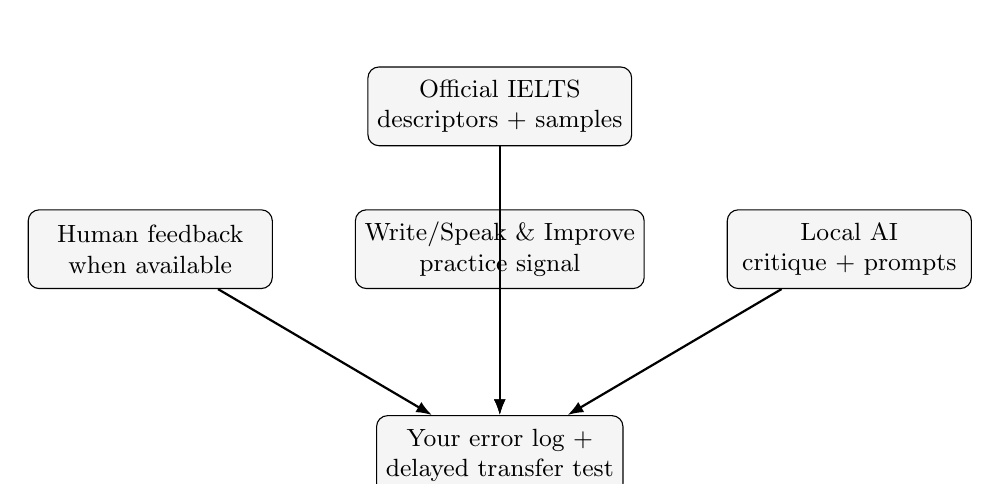
\begin{tikzpicture}[node distance=8mm and 12mm, every node/.style={font=\small}, box/.style={draw,rounded corners,align=center,minimum width=3.1cm,minimum height=1.0cm,fill=gray!8}, arrow/.style={-{Latex[length=2mm]},thick}]
\node[box] (official) {Official IELTS\\descriptors + samples};
\node[box, below left=of official] (human) {Human feedback\\when available};
\node[box, below=of official] (awe) {Write/Speak \& Improve\\practice signal};
\node[box, below right=of official] (localai) {Local AI\\critique + prompts};
\node[box, below=16mm of awe] (learner) {Your error log +\\delayed transfer test};
\draw[arrow] (official)--(learner);
\draw[arrow] (human)--(learner);
\draw[arrow] (awe)--(learner);
\draw[arrow] (localai)--(learner);
\end{tikzpicture}
\end{center}

\begin{warningbox}[AI score warning]
Automated feedback is useful, but the evidence does not justify treating a chatbot or automated writing/speaking score as an IELTS examiner. A 2023 meta-analysis found a medium average effect for automated writing feedback but substantial heterogeneity. A 2026 meta-analysis of AI-assisted L2 writing feedback found a modest overall effect, with larger emotional/engagement effects than cognitive gains. Another 2026 synthesis highlighted weak transfer in some algorithm-based feedback research.\src{12}\src{13} Use AI to create \textbf{more and better practice}, not to certify your band.
\end{warningbox}

\section{Free AI Workflows That Actually Help}

\subsection{Local AI setup}
For the strict zero-payment path, run a local language model with llama.cpp. Qwen3-4B is published with an Apache-2.0 license and is small enough for many modern computers; stronger local models require more memory.\src{27}\src{28} If your computer cannot run a suitable model, skip the local AI step rather than switching to a trial/credit-based service.

\subsection{Prompt 1: rubric evidence extraction}
\begin{aibox}[Paste into a local LLM]
\small
You are a diagnostic writing coach, not an IELTS examiner. I will give you the official IELTS Writing descriptors and my essay. Do not give a final band first. For each of the four criteria: (1) quote or paraphrase 2-4 specific pieces of evidence from my essay, (2) identify the strongest feature, (3) identify the single highest-impact weakness, (4) propose one revision exercise. Distinguish task/content problems from language errors. After that, give only a broad range and explain uncertainty. Do not invent IELTS rules not present in the rubric.
\end{aibox}

\subsection{Prompt 2: Task Response adversary}
\begin{aibox}[Argument stress test]
\small
Read my IELTS Task 2 plan. Act as a skeptical reader. List every obligation in the prompt. Then test whether each body paragraph directly helps answer one of those obligations. For each main idea, ask: Why? By what mechanism? Under what conditions? What concrete example would make it specific? What counterexample or limitation could weaken it? Do not rewrite the essay for me; force me to supply the missing reasoning.
\end{aibox}

\subsection{Prompt 3: speaking transcript analyzer}
\begin{aibox}[Speaking diagnosis]
\small
Here is a transcript of my 5-minute speaking sample. Ignore pronunciation because you do not have the audio. Tag: [G] grammar, [C] collocation/word choice, [V] vague/repetitive vocabulary, [D] discourse/coherence, [F] filler/restart. Count recurring error families. Choose only the top two targets for the next session. Then generate five new Part 3 questions that force me to use the corrected structures without repeating the same content.
\end{aibox}

\subsection{Prompt 4: rewrite comparison without plagiarism}
\begin{aibox}[Revision audit]
\small
Compare Draft A and Draft B. Do not praise style generally. Identify exactly which changes improved task fulfillment, coherence, lexical precision, or grammar, and which changes merely made the wording more complicated. Flag any sentence that became less natural. Then propose three principles I should transfer to a completely new essay.
\end{aibox}

\section{Evidence-Based Practice Principles}

\subsection{Feedback must cause revision}
A 2024 meta-analysis across L1/L2/foreign-language writing found that surface feedback improved surface outcomes, deep feedback improved deep outcomes, and combined feedback improved both.\src{11} The practical implication is simple: do not use a grammar checker only to produce a cleaner final draft. Convert its feedback into a rule, an error log entry, and a delayed new-task test.

\subsection{Automated feedback is supplementary}
Meta-analytic evidence on automated writing evaluation is positive on average but heterogeneous.\src{12}\src{13} At an advanced level, this means AI is particularly useful for volume, categorization, and generating transfer tasks; it is less trustworthy for subtle judgments such as whether an argument is fully developed at Band 9 or whether a lexical choice is optimally idiomatic in context.

\subsection{Task repetition helps speaking -- if you test transfer}
A 2025 meta-analysis reports positive effects of task repetition across oral performance dimensions.\src{14} The critical safeguard is to follow repeated performance with a novel prompt. Otherwise improved fluency may partly reflect familiarity with the content rather than a more general skill.

\section{Twelve-Month Writing + Speaking Plan}

\begin{figure}[H]
\centering
\includegraphics[width=0.94\textwidth]{year_workload.png}
\caption{Proposed weekly active workload. These are planning targets, not claims about a required number of hours.}
\end{figure}

\begin{figure}[H]
\centering
\includegraphics[width=0.94\textwidth]{readiness_timeline.png}
\caption{Illustrative readiness targets. Band-equivalent practice ratings are inherently noisy; use trends across multiple samples.}
\end{figure}

\subsection{Months 1-3: diagnosis and accuracy}
Weekly minimum:
\begin{itemize}
\item 2 Task 2 essays using the full feedback-rewrite-transfer cycle;
\item 2 Task 1 overview drills + 1 full Task 1;
\item 3 speaking sessions of 25-35 minutes;
\item 1 full speaking mock every two weeks;
\item 1 weekly error-log review.
\end{itemize}
Milestone: eliminate the top three recurring grammar/collocation error families from revised work and cut their frequency substantially in unseen tasks.

\subsection{Months 4-6: development and precision}
Increase idea-development drills, corpus work, and Part 3 abstract discussion. Start blind self-rating before using automated feedback. Once per week, take an old essay and produce a completely new essay on the same broad theme without looking at the old wording.

Milestone: timed Writing samples should consistently satisfy Band 8 descriptors in all four criteria according to your rubric evidence, not just receive a single optimistic score.

\subsection{Months 7-9: spontaneous transfer}
Reduce same-task repetition and increase new-task transfer. For speaking, rotate unfamiliar abstract topics. For writing, use prompts that differ in logical structure. Every two weeks run a ``cold'' mini-exam: unseen Task 1 + Task 2 under exact time limits and no tools.

Milestone: most samples show no obvious Band 7 limiting feature; weaknesses are occasional rather than systematic.

\subsection{Months 10-11: exam integration}
Do one full Writing paper and one full Speaking mock each week. Other sessions become targeted repair. Maintain Reading/Listening with occasional checks rather than intensive study if they remain stable.

Milestone: a rolling set of at least 6-8 independent productive samples is at/above the strategic threshold you need, preferably with a cushion.

\subsection{Month 12: taper and stability}
Decrease new theory. Practice under realistic timing, sleep schedule, keyboard/paper format, and test conditions. Use the last two weeks to protect consistency rather than chase new vocabulary.

\section{A Weekly Schedule for the Advanced Learner}

\begin{table}[H]
\centering
\begin{tabularx}{\textwidth}{p{1.6cm}X X}
\toprule
Day & Main block (45-70 min) & Secondary block (20-35 min) \\
\midrule
Mon & Task 2 timed draft + self-rubric & Speaking Part 3 cold questions \\
Tue & Feedback + repair + rewrite & SKELL/Lextutor collocation review \\
Wed & Academic Task 1 overview drills + one full report & Part 2 record-transcribe-repeat \\
Thu & New Task 2 transfer prompt & Grammar error-family drills \\
Fri & Speaking 4/3/2 + new transfer question & Listen back and code transcript \\
Sat & Alternating full Writing paper / full Speaking mock & Weekly error-log review \\
Sun & Light native-level reading/listening only & Optional Anki review; no heavy IELTS work \\
\bottomrule
\end{tabularx}
\end{table}

\section{The Final 8 Weeks: Probability-Maximization Protocol}

\subsection{Weeks 8-5 before test}
\begin{itemize}
\item 1 full Writing paper/week, 1 additional Task 2, 1 Task 1 micro-session.
\item 1 full Speaking mock/week, plus 2 short focused speaking sessions.
\item Continue error-log transfer tests.
\item Score trends using the same rubric and the same evidence method.
\end{itemize}

\subsection{Weeks 4-3}
Increase exam-condition simulations to two productive mock blocks per week, but preserve review quality. Stop collecting large amounts of new vocabulary. Focus on reliability: prompt interpretation, overview selection, idea depth, grammar under time pressure, and natural spoken topic development.

\subsection{Week 2}
One or two final full simulations early in the week. Then reduce volume by roughly one third. Review only recurring error families and proven strategies.

\subsection{Final week}
No marathon study. Do short warm-ups, one light Task 1 overview, one Task 2 plan, and several 5-minute speaking bursts. The objective is stable retrieval, not last-minute expansion.

\begin{warningbox}[Do not use a single mock as proof of readiness]
A single 9-level performance can be a lucky prompt. A single 7.5 can be an unlucky one. Readiness is a \textbf{distribution}: multiple unseen tasks, different topics, timed conditions, and ideally more than one evaluator or feedback channel.
\end{warningbox}

\section{Band 9 Readiness Scorecard}

\subsection{Writing}
Rate each item 0 (not reliable), 1 (inconsistent), 2 (reliable):
\begin{longtable}{p{0.78\textwidth}p{0.12\textwidth}}
\toprule
Check & 0/1/2 \\
\midrule
I identify every obligation in a Task 2 prompt before writing. & \\
My position remains consistent and directly answers the question. & \\
Each main idea is extended with mechanism/detail, not just assertion. & \\
Paragraph progression is clear without depending on visible linkers. & \\
I use precise collocations and can verify doubtful phrases in a corpus. & \\
My top three grammar errors are rare in unseen timed essays. & \\
My Task 1 overview selects dominant features rather than listing data. & \\
I finish both tasks with time for verification. & \\
I can reproduce high-quality performance on a new prompt 3-5 days later. & \\
\bottomrule
\end{longtable}

\subsection{Speaking}
\begin{longtable}{p{0.78\textwidth}p{0.12\textwidth}}
\toprule
Check & 0/1/2 \\
\midrule
My pauses are mostly content-planning pauses rather than word-search breakdowns. & \\
I can sustain Part 2 for close to two minutes without padding. & \\
I develop Part 3 answers with reasons, examples, and qualifications. & \\
I can paraphrase when a word is unavailable without obvious panic. & \\
My recurring grammar errors are uncommon in spontaneous speech. & \\
I can discuss abstract unfamiliar topics, not only practiced themes. & \\
My speech remains easy to understand under time pressure. & \\
A new topic after repetition still shows the improvement. & \\
\bottomrule
\end{longtable}

\section{Printable Error Logs}

\subsection{Writing error log}
\begin{longtable}{p{2cm}p{3.1cm}p{3.1cm}p{3.4cm}p{2.2cm}}
\toprule
Date & Error/weakness & Correct principle & Transfer task & Resolved? \\
\midrule
\endfirsthead
\toprule
Date & Error/weakness & Correct principle & Transfer task & Resolved? \\
\midrule
\endhead
& & & & \\
\addlinespace[8mm]
& & & & \\
\addlinespace[8mm]
& & & & \\
\addlinespace[8mm]
& & & & \\
\bottomrule
\end{longtable}

\subsection{Speaking error log}
\begin{longtable}{p{2cm}p{2.2cm}p{3cm}p{3.5cm}p{2.6cm}}
\toprule
Date & Code (F/W/G/C/D/P) & Example & Repair drill & New-task result \\
\midrule
& & & & \\
\addlinespace[8mm]
& & & & \\
\addlinespace[8mm]
& & & & \\
\addlinespace[8mm]
& & & & \\
\bottomrule
\end{longtable}

\section{What To Do This Week}

\begin{practicebox}[Seven-day launch protocol]
\textbf{Day 1:} Download the current IELTS Writing and Speaking descriptors; complete one unseen Task 2 and one 11-14 minute speaking mock.\\
\textbf{Day 2:} Self-rate both using evidence, then run the writing through Write \& Improve and the speech through Speak \& Improve. Save the original before editing.\\
\textbf{Day 3:} Build the first error log. Pick two writing errors and two speaking errors only.\\
\textbf{Day 4:} Rewrite the essay from a blank page; verify 5 doubtful collocations in SKELL.\\
\textbf{Day 5:} Repeat one Part 2/3 speaking task, transcribe it with whisper.cpp, then answer a new related question.\\
\textbf{Day 6:} Do one Academic Task 1 overview-only set (5 charts) and one 30-minute Part 3 session on abstract topics.\\
\textbf{Day 7:} Review the log, create 10-20 Anki cards from your actual errors/collocations, and stop. No new material.
\end{practicebox}

\section{Source Quality Hierarchy}

Use sources in this order when they disagree:
\begin{enumerate}
\item Official IELTS scoring rules, descriptors, sample tasks, and examiner comments.
\item Peer-reviewed meta-analyses/systematic reviews on feedback, automated evaluation, and task repetition.
\item University/research-project tools such as Cambridge Write \& Improve and Speak \& Improve.
\item Corpora and open-access academic writing resources.
\item Open-source software documentation.
\item AI-generated suggestions only after checking them against the layers above.
\end{enumerate}

\section{References and Direct Links}
\small
\begin{enumerate}[label={[R\arabic*]},leftmargin=2.4em]
\item IELTS. \textit{IELTS scoring in detail: band scores explained}. \url{https://ielts.org/take-a-test/your-results/ielts-scoring-in-detail}
\item IELTS. \textit{Speaking Band Descriptors}. \url{https://ielts.org/cdn/ielts-guides/ielts-speaking-band-descriptors.pdf}
\item IELTS. \textit{Writing Band Descriptors}. \url{https://ielts.org/cdn/ielts-guides/ielts-writing-band-descriptors.pdf}
\item IELTS. \textit{Writing key assessment criteria}. \url{https://ielts.org/cdn/ielts-guides/ielts-writing-key-assessment-criteria.pdf}
\item IELTS. \textit{Writing test preparation resources}. \url{https://ielts.org/take-a-test/preparation-resources/writing-test-resources}
\item IELTS. \textit{Speaking key assessment criteria}. \url{https://ielts.org/cdn/ielts-guides/ielts-speaking-key-assessment-criteria.pdf}
\item IELTS. \textit{IELTS Academic sample test questions}. \url{https://ielts.org/take-a-test/preparation-resources/sample-test-questions/academic-test}
\item IELTS. \textit{Academic Writing sample tasks and examiner comments}. \url{https://ielts.org/cdn/Sample-tests/ielts-academic-writing-sample-tasks-2023.pdf}
\item British Council. \textit{Free IELTS Academic Writing practice tests}. \url{https://takeielts.britishcouncil.org/prepare/ielts-free-practice-mock-tests/academic/writing}
\item British Council. \textit{Free IELTS Academic Speaking practice tests}. \url{https://takeielts.britishcouncil.org/prepare/ielts-free-practice-mock-tests/academic/speaking}
\item Scherer, S., Graham, S., \& Busse, V. (2024). \textit{How effective is feedback for L1, L2, and FL learners' writing? A meta-analysis}. Learning and Instruction, 93, 101961. \url{https://doi.org/10.1016/j.learninstruc.2024.101961}
\item Fleckenstein, J., Liebenow, L., \& Meyer, J. (2023). \textit{Automated feedback and writing: a multi-level meta-analysis of effects on students' performance}. Frontiers in Artificial Intelligence. \url{https://doi.org/10.3389/frai.2023.1162454}
\item \textit{The effects of AI-assisted feedback on students' perceptions, emotions, and learning outcomes in L2 writing: a three-level meta-analysis} (2026). System, 139, 104018. \url{https://doi.org/10.1016/j.system.2026.104018}
\item \textit{Task repetition and L2 oral performance: A meta-analysis} (2025). System, 135, 103868. \url{https://doi.org/10.1016/j.system.2025.103868}
\item Guo, J., \& Saito, K. (2026). \textit{Effects of the 4/3/2 activity revisited: Aptitude matters, but distributed practice does not}. System, 137, 103936. \url{https://doi.org/10.1016/j.system.2025.103936}
\item Cambridge. \textit{Write \& Improve}. \url{https://writeandimprove.com/free}
\item Cambridge. \textit{Write \& Improve - free resources page}. \url{https://www.cambridgeenglish.org/learning-english/free-resources/write-and-improve/}
\item Cambridge. \textit{Speak \& Improve}. \url{https://speakandimprove.com/}
\item Sketch Engine. \textit{SKELL - examples and collocations for learners of English}. \url{https://www.sketchengine.eu/skell/}
\item Cobb, T. \textit{Compleat Lexical Tutor}. \url{https://www.lextutor.ca/}
\item University of Manchester. \textit{Academic Phrasebank}. \url{https://www.phrasebank.manchester.ac.uk/}
\item Automattic. \textit{Harper: offline, open-source grammar checker}. \url{https://github.com/Automattic/harper}
\item LanguageTool. \textit{Open-source LanguageTool core}. \url{https://github.com/languagetool-org/languagetool}
\item ggml-org. \textit{whisper.cpp}. \url{https://github.com/ggml-org/whisper.cpp}
\item Audacity Team. \textit{Audacity}. \url{https://www.audacityteam.org/download/}
\item Boersma, P., Weenink, D., \& Shchupak, A. \textit{Praat: doing phonetics by computer}. \url{https://praat.org/}
\item ggml-org. \textit{llama.cpp}. \url{https://github.com/ggml-org/llama.cpp}
\item Qwen. \textit{Qwen3-4B model card, Apache 2.0}. \url{https://huggingface.co/Qwen/Qwen3-4B}
\item Anki. \textit{Anki desktop and mobile availability}. \url{https://apps.ankiweb.net/}
\end{enumerate}

\vfill
\begin{evidencebox}[Bottom line]
The shortest credible route is not ``study more IELTS.'' It is: \textbf{official rubric -> timed output -> evidence-based diagnosis -> focused repair -> rewrite/re-speak -> delayed unseen transfer -> repeated mock distribution}. Keep the free tools subordinate to that loop. If Reading and Listening remain at 9, reliable 8.5-level Writing and Speaking is mathematically enough for an overall 9, but build a safety margin because no score can be guaranteed in advance.
\end{evidencebox}

\end{document}
